\documentclass{beamer}
\usepackage{epstopdf}
\usepackage{tabularx}
\usepackage{adjustbox}
\usepackage{pdflscape}
\usepackage[]{hyperref}
\definecolor{links}{HTML}{0B610B} % dark green
%\definecolor{links}{HTML}{2A1B81} % dark blue
\hypersetup{colorlinks,linkcolor=,urlcolor=links}
\usepackage{multirow} % for tables
\usepackage{multicol}
\usepackage{subfig}
\usepackage{graphicx}
\usetheme{Madrid}
\title[Hashing classification for tracking ]{Hashing Classification for charged particle tracking}
\author[Luiza Adelina Ciucu (ATLAS) ]{Luiza Adelina Ciucu (ATLAS)} 

\titlegraphic{
%
\includegraphics[height=2.1cm]{./physics_section_EN_q.eps} 

\includegraphics[height=2.1cm]{./physics_section_EN_q-eps-converted-to.pdf} 
}

\date{10 July 2020}

\pdfsuppresswarningpagegroup=1

\begin{document}

\frame{\titlepage}

%\texttt{\detokenize{

% define input folder for our plots only once
\newcommand\inputFolderMerge{../output_new_ev_000_100_min_10}
\newcommand\inputFolderMergedBalanced{../output_new_ev_000_100_min_10_balanced17}
\newcommand\inputFolderNN{../output_new_ev_000_100_min_10_NN_07}
\newcommand\inputFolderOverlay{../output_overlay_balanced_ev_000_100_Min10_17_B}

% add some useful definitions
%\def\MeV{\ifmmode {\mathrm{\ Me\kern -0.1em V}}\else
%                   \textrm{Me\kern -0.1em V}\fi}%  

\def\volumeID{\texttt{\detokenize{volume_id}}}
\def\layerID{\texttt{\detokenize{layer_id}}}

\def\TP{\ifmmode {\mathrm{TP}}\else
                   \textrm{TP}\fi}%
\def\FP{\ifmmode {\mathrm{FP}}\else
                   \textrm{FP}\fi}%                                     
\def\FN{\ifmmode {\mathrm{FN}}\else
                   \textrm{FN}\fi}%
\def\TN{\ifmmode {\mathrm{TN}}\else
                   \textrm{TN}\fi}%

\def\Ni{\ifmmode {\mathrm{N}_\mathrm{i}}\else
                   \textrm{N}_{\textrm{i}}\fi}%
\def\wi{\ifmmode {\mathrm{w}_\mathrm{i}}\else
                   \textrm{w}_{\textrm{i}}\fi}%
\def\xi{\ifmmode {\mathrm{x}_\mathrm{i}}\else
                   \textrm{x}_{\textrm{i}}\fi}%
\def\wzero{\ifmmode {\mathrm{w}_\mathrm{0}}\else
                   \textrm{w}_{\textrm{0}}\fi}%
\def\xzero{\ifmmode {\mathrm{x}_\mathrm{0}}\else
                   \textrm{x}_{\textrm{0}}\fi}%
                   


% intro slide
\begin{frame}{Introduction}
\begin{enumerate}
\item[o] 100 events. For each group of 10: 7 train, 3 test.  
\item[o] If nbPositiveHit$<$10, set nbPositiveHit=0 and output made only of -1.
\item[o] For Train used Balanced (130k), for Test use Unbalanced (3.2M).
\item[o] Balancing Train in two steps, as shown last time.
\begin{enumerate}
\item[-] Make peak flat between 10-17 (with value of 17).
\item[-] Reduce nbPositiveHit=0 until 50\% Pos, 50\% Neg.
\end{enumerate}
\item[o] Train in Balanced, evaluate in Test in Unbalanced.
\item[o] Last time showed how peak at 17 gives best results.
 \begin{enumerate}
\item[-] Many values at bin, and almost nothing at bins 1-9 (out of 21)
\item[-] But problem that only a peak in 1-2 bins around bin 14.
\end{enumerate}
\item[o] New studies today:
 \begin{enumerate}
\item[-] Tried other model settings.
\item[-] Also added a dropout(0.2) layer at the end of the hidden layers.
\end{enumerate}
\end{enumerate}
\end{frame}
\clearpage

\begin{frame}{Model changes}
\begin{enumerate}
\item[o] Naming convention of model description, e,g. \texttt{\detokenize{02_05_E_RH_A_0120}}.
\begin{enumerate}
\item[-] 02 hidden layers
\item[-] 05 x 20 nodes on the hidden layer. \\ Input layer has 3 x 20 nodes, output layer has 1 x 20 nodes.
\item[-] E = elu activation function for all nodes on all the hidden layers. \\ Other options: R = relu.
\item[-] RH = regular hinge loss function (power one). \\ Other options: SH = squared hinge loss function (power two).
\item[-] A = no dropout layer at the end of hidden layers. \\ Option options: B = one dropout layer at the end of the hidden layers.
\item[-] 0120 number of epochs, each with batch size of 50000. \\ Other options: 600, 1200. 
\end{enumerate}
\item[o] Today they all have Tanh activation function on the output layer. \\ Squared non linear and soft sign were not that good.
\item[o] Comparing best models from last week with the best models from this week.
\end{enumerate}
\end{frame}
\clearpage

\begin{frame}{Accuracy and Loss from training}
\begin{enumerate}
\item[o] For 120 epochs, Test shows unbalanced, for 1200 Test balanced.
\end{enumerate}
\includegraphics[width=0.45\textwidth]{\inputFolderOverlay/plot_01_1_overlay_graph_accuracyBinary_Train.pdf}
\includegraphics[width=0.45\textwidth]{\inputFolderOverlay/plot_01_1_overlay_graph_loss_Train.pdf} \\
\includegraphics[width=0.45\textwidth]{\inputFolderOverlay/plot_01_1_overlay_graph_accuracyBinary_Test.pdf}
\includegraphics[width=0.45\textwidth]{\inputFolderOverlay/plot_01_1_overlay_graph_loss_Test.pdf}
\end{frame}
\clearpage





\begin{frame}{Output and output predicted 1D}
\begin{enumerate}
\item[o] Older ones have a sharp peak, the new ones are more flat. 
\end{enumerate}
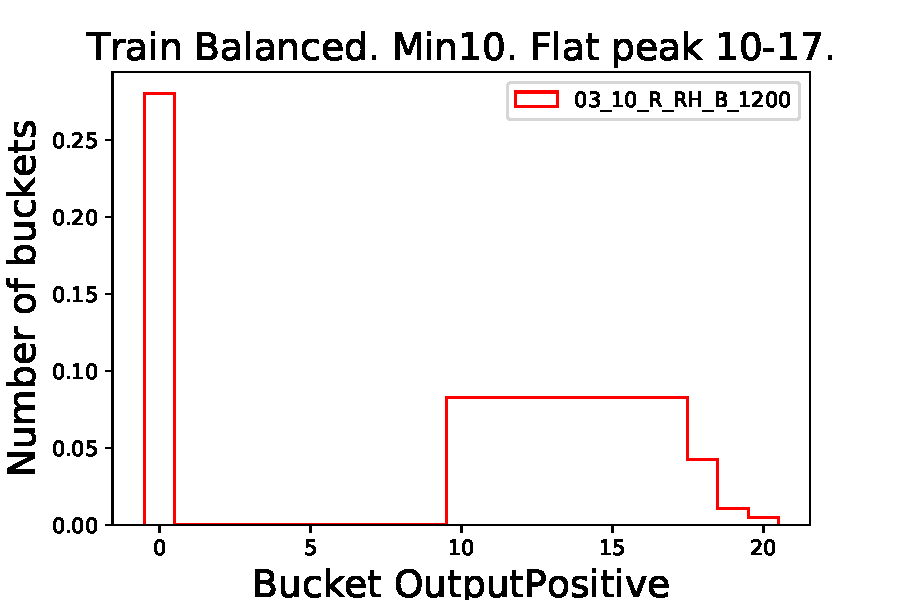
\includegraphics[width=0.45\textwidth]{\inputFolderOverlay/plot_02_1_overlay_histo_OutputPositive_Train.pdf}
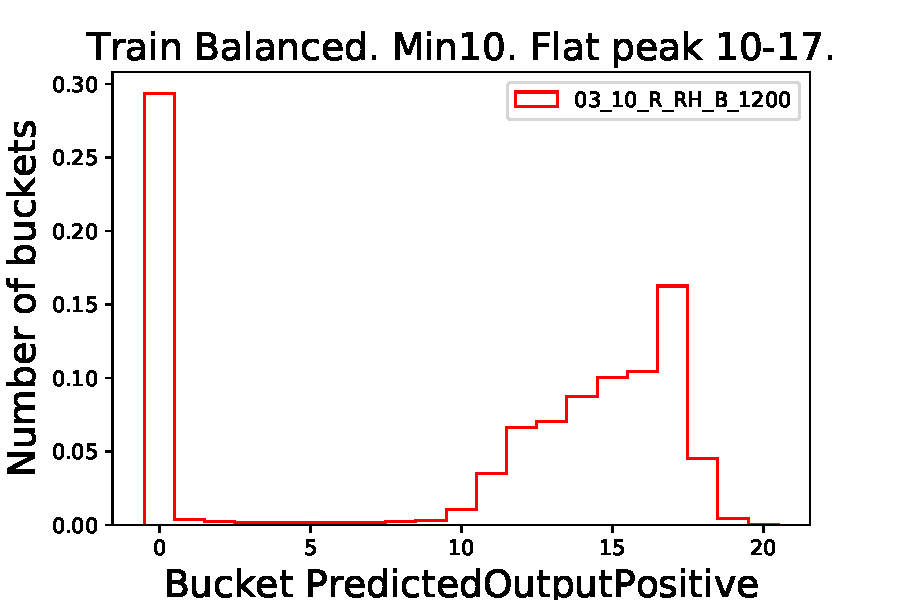
\includegraphics[width=0.45\textwidth]{\inputFolderOverlay/plot_02_1_overlay_histo_PredictedOutputPositive_Train.pdf}\\
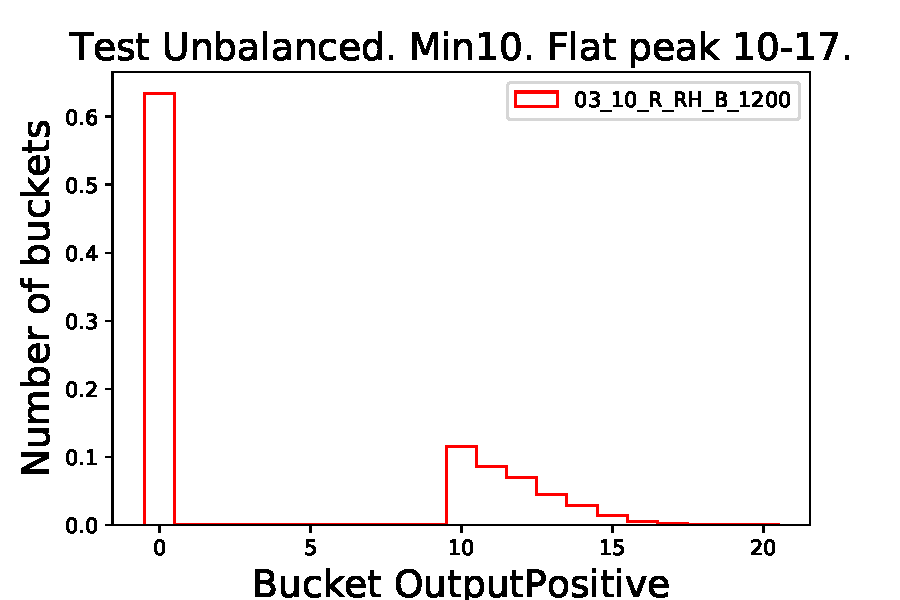
\includegraphics[width=0.45\textwidth]{\inputFolderOverlay/plot_02_1_overlay_histo_OutputPositive_Test.pdf}
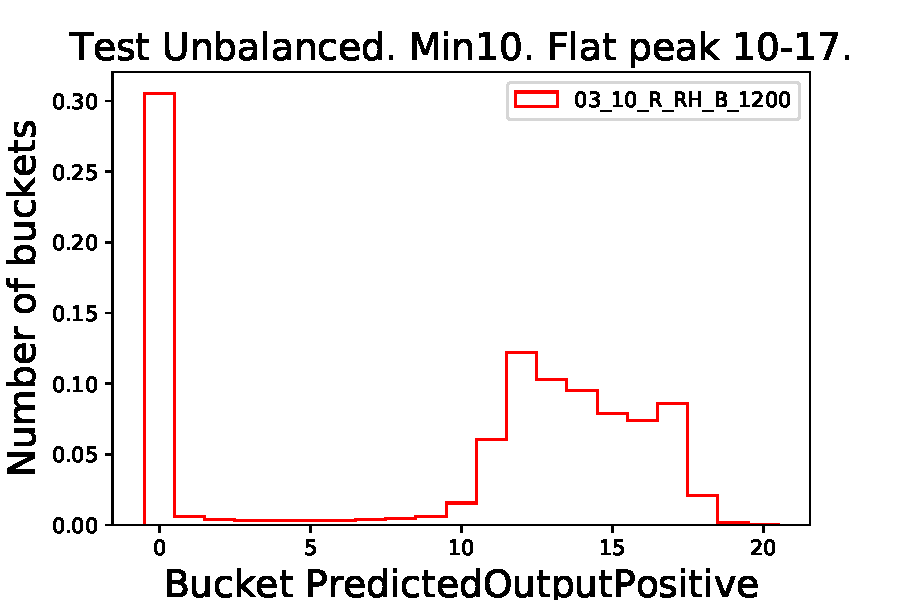
\includegraphics[width=0.45\textwidth]{\inputFolderOverlay/plot_02_1_overlay_histo_PredictedOutputPositive_Test.pdf}
\end{frame}
\clearpage

\begin{frame}{Output and output predicted 2D 1/2 - last week}
\begin{enumerate}
\item[o] No diagonal in either Train or Test. 
\end{enumerate}
\includegraphics[width=0.45\textwidth]{\inputFolderOverlay/plot_04_1_overlay_histo2D_OutputPositive_PredictedOutputPositive_02_05_E_RH_A_0120_Train.pdf}
\includegraphics[width=0.45\textwidth]{\inputFolderOverlay/plot_04_1_overlay_histo2D_OutputPositive_PredictedOutputPositive_02_05_E_SH_A_0120_Train.pdf}\\
\includegraphics[width=0.45\textwidth]{\inputFolderOverlay/plot_04_1_overlay_histo2D_OutputPositive_PredictedOutputPositive_02_05_E_RH_A_0120_Test.pdf}
\includegraphics[width=0.45\textwidth]{\inputFolderOverlay/plot_04_1_overlay_histo2D_OutputPositive_PredictedOutputPositive_02_05_E_SH_A_0120_Test.pdf}\\
\end{frame}
\clearpage

\begin{frame}{Output and output predicted 2D 2/2 - new models}
\begin{enumerate}
\item[o] In Train balanced, a diagonal is seen. In Test unbalanced it's harder.
\end{enumerate}
\includegraphics[width=0.45\textwidth]{\inputFolderOverlay/plot_04_1_overlay_histo2D_OutputPositive_PredictedOutputPositive_03_10_E_SH_B_1200_Train.pdf}
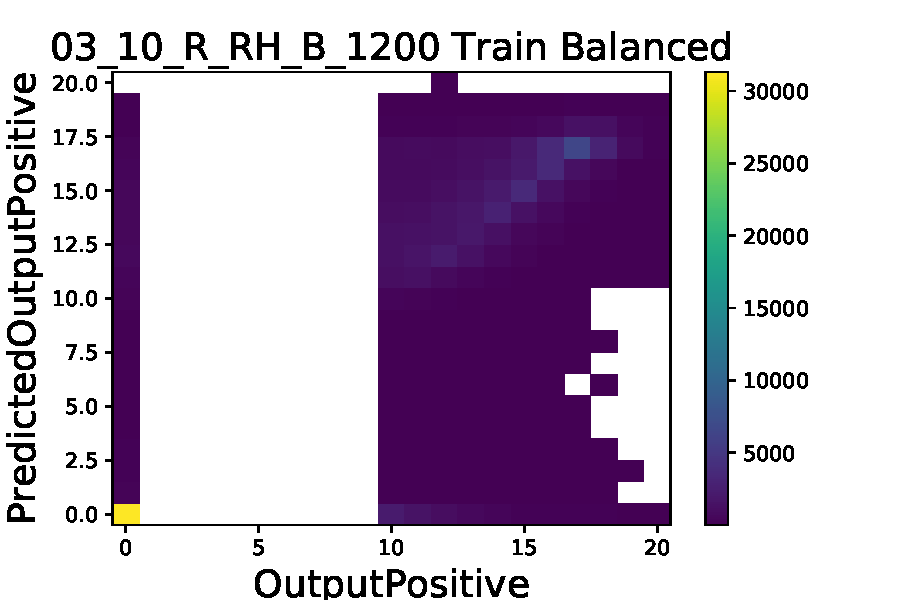
\includegraphics[width=0.45\textwidth]{\inputFolderOverlay/plot_04_1_overlay_histo2D_OutputPositive_PredictedOutputPositive_03_10_R_RH_B_1200_Train.pdf}\\
\includegraphics[width=0.45\textwidth]{\inputFolderOverlay/plot_04_1_overlay_histo2D_OutputPositive_PredictedOutputPositive_03_10_E_SH_B_1200_Test.pdf}
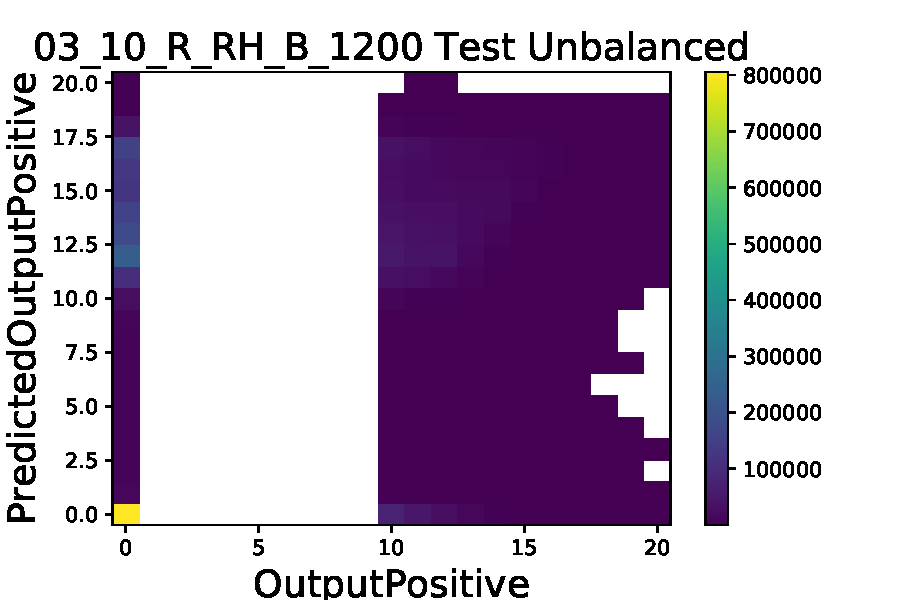
\includegraphics[width=0.45\textwidth]{\inputFolderOverlay/plot_04_1_overlay_histo2D_OutputPositive_PredictedOutputPositive_03_10_R_RH_B_1200_Test.pdf}\\
\end{frame}
\clearpage

\begin{frame}{Metrics for each VolumeID.}
\begin{enumerate}
\item[o] The new ones (bluish) have a clearly better Train Balance and only a slightly better Test Unbalanced than the old ones (reddish).
\end{enumerate}
\centering
% table
\begin{center}
\begin{tabular}{ |c|c|c| } 
\hline
Accuracy & Precision & Recall \\ 
\hline
$\frac{\TP+\TN}{\TP+\FP+\FN+\TN}$ & $\frac{\TP}{\TP+\FP}$  & $\frac{\TP}{\TP+\FN}$ \\ 
\hline
\end{tabular}
\end{center}
% plots
\includegraphics[width=0.32\textwidth]{\inputFolderOverlay/plot_03_1_overlay_graph_Accuracy_VolumeID_Train.pdf}
\includegraphics[width=0.32\textwidth]{\inputFolderOverlay/plot_03_1_overlay_graph_Precision_VolumeID_Train.pdf}
\includegraphics[width=0.32\textwidth]{\inputFolderOverlay/plot_03_1_overlay_graph_Recall_VolumeID_Train.pdf}\\
% plots
\includegraphics[width=0.32\textwidth]{\inputFolderOverlay/plot_03_1_overlay_graph_Accuracy_VolumeID_Test.pdf}
\includegraphics[width=0.32\textwidth]{\inputFolderOverlay/plot_03_1_overlay_graph_Precision_VolumeID_Test.pdf}
\includegraphics[width=0.32\textwidth]{\inputFolderOverlay/plot_03_1_overlay_graph_Recall_VolumeID_Test.pdf}\\
\end{frame}

\begin{frame}{Conclusion}
\begin{enumerate}
\item[o] Improved model from last week.
\item[o] In balanced dataset (Train and Test) a diagonal can be nicely seen.
\item[o] In Test unbalanced it is harder to see, \\ but still values look relatively flat in 1D. 
\item[o] Changes to the model for the best choice: \\ \texttt{\detokenize{02_05_E_SH_A_0120}} $\rightarrow$ \texttt{\detokenize{03_10_R_RH_B_1200}}.
\begin{enumerate}
\item[-] 02 $\rightarrow$ 03 hidden layers
\item[-] 05 x 20 $\rightarrow$ 10 x 20 nodes on each hidden layer. \\ Input layer has 3 x 20 nodes, output layer has 1 x 20 nodes.
\item[-] Elu $\rightarrow$ Relu activation function for all nodes on all the hidden layers. 
\item[-] Squared Hinge $\rightarrow$ Regular Hinge as loss function.
\item[-] Added one dropout layer (0.2) at the end of the hidden layers.
\item[-] 120 $\rightarrow$ 1200 epochs, each with batch size of 50000.
\item[-] Kept Tanh activation function on the output layer.
\end{enumerate}
\item[o] This model seems good enough.
\item[o] Next step: add these results in the thesis. 
\end{enumerate}
\end{frame}
\clearpage

\end{document}

\begin{frame}{2D plots TANH SH 50}
\includegraphics[width=0.49\textwidth]{\inputFolderNN/NN_5_Balanced17_TANH_SH_50_50000_histo_OutputPositive.pdf}
\includegraphics[width=0.49\textwidth]{\inputFolderNN/NN_5_Balanced17_TANH_SH_50_50000_histo_PredictedOutputPositive.pdf}\\
\includegraphics[width=0.49\textwidth]{\inputFolderNN/NN_5_Balanced17_TANH_SH_50_50000_histo_OutputPositive_vs_PredictedOutputPositive_Train.pdf}
\includegraphics[width=0.49\textwidth]{\inputFolderNN/NN_5_Balanced17_TANH_SH_50_50000_histo_OutputPositive_vs_PredictedOutputPositive_Test.pdf}
\end{frame}
\clearpage



\begin{frame}{2D plots SQNL SH 50}
\includegraphics[width=0.49\textwidth]{\inputFolderNN/NN_5_Balanced17_SQNL_SH_50_50000_histo_OutputPositive.pdf}
\includegraphics[width=0.49\textwidth]{\inputFolderNN/NN_5_Balanced17_SQNL_SH_50_50000_histo_PredictedOutputPositive.pdf}\\
\includegraphics[width=0.49\textwidth]{\inputFolderNN/NN_5_Balanced17_SQNL_SH_50_50000_histo_OutputPositive_vs_PredictedOutputPositive_Train.pdf}
\includegraphics[width=0.49\textwidth]{\inputFolderNN/NN_5_Balanced17_SQNL_SH_50_50000_histo_OutputPositive_vs_PredictedOutputPositive_Test.pdf}
\end{frame}
\clearpage

\begin{frame}{2D plots SOSI SH 50}
\includegraphics[width=0.49\textwidth]{\inputFolderNN/NN_5_Balanced17_SOSI_SH_50_50000_histo_OutputPositive.pdf}
\includegraphics[width=0.49\textwidth]{\inputFolderNN/NN_5_Balanced17_SOSI_SH_50_50000_histo_PredictedOutputPositive.pdf}\\
\includegraphics[width=0.49\textwidth]{\inputFolderNN/NN_5_Balanced17_SOSI_SH_50_50000_histo_OutputPositive_vs_PredictedOutputPositive_Train.pdf}
\includegraphics[width=0.49\textwidth]{\inputFolderNN/NN_5_Balanced17_SOSI_SH_50_50000_histo_OutputPositive_vs_PredictedOutputPositive_Test.pdf}
\end{frame}
\clearpage

\begin{frame}{Study 2: varying number of epochs}
\begin{enumerate}
\item[o] Conclusions:
\item[o] 120 vs 50 epochs.
\item[o] Looking at 120 epochs it appeared that from 50 epochs it started to overtrain.
\item[o] So ran again with 50 epochs. 
\item[o] But results look a bit worse, including for Test. 
\end{enumerate}
\end{frame}
\clearpage

% intro slide
\begin{frame}{Conclusion}
\begin{enumerate}
\item[o] 100 events. For each group of 10: 7 train, 3 test.  
\item[o] If nbPositiveHit$<$10, set nbPositiveHit=0 and output made only of -1.
\item[o] For Train used Balanced (130k), for Test use Unbalanced (3.2M).
\item[o] Balancing Train in two steps, as shown last time.
\begin{enumerate}
\item[-] Make peak flat between 10-17 (with value of 17).
\item[-] Reduce nbPositiveHit=0 until 50\% Pos, 50\% Neg.
\end{enumerate}
\item[o] New studies today
 \begin{enumerate}
\item[-] Last time Test was also Balanced. Now Test is Unbalanced.
\item[-] With constraint of our output of -1 and 1: 
\item[-] Very similar with various layer activation functions: tanh, squared non linear, soft sign.
\item[-] Very similar with various loss functions: squared hinge and hinge.
\item[-] Overtrain at 50 epochs maybe a false alarm? As 50 epochs slight worse than 120 epochs. Try 120 epochs vs 50 epochs.
\end{enumerate}
\end{enumerate}
\end{frame}
\clearpage





\begin{frame}{Study 3: for 120 epochs, vary loss function}
\begin{enumerate}
\item[o] Squared hinge, Hinge. 
\end{enumerate}
\end{frame}
\clearpage

\begin{frame}{Accuracy and Loss from training}
\includegraphics[width=0.49\textwidth]{\inputFolderOverlay_04/plot_01_1_overlay_graph_accuracyBinary_Train.pdf}
\includegraphics[width=0.49\textwidth]{\inputFolderOverlay_04/plot_01_1_overlay_graph_accuracyBinary_Test.pdf}\\
\includegraphics[width=0.49\textwidth]{\inputFolderOverlay_04/plot_01_1_overlay_graph_loss_Train.pdf}
\includegraphics[width=0.49\textwidth]{\inputFolderOverlay_04/plot_01_1_overlay_graph_loss_Test.pdf}
\end{frame}
\clearpage

\begin{frame}{Metrics for each VolumeID.}
\begin{enumerate}
\item[o] Squared hinge vs hinge quite similar. 
\end{enumerate}
\centering
% table
\begin{center}
\begin{tabular}{ |c|c|c| } 
\hline
Accuracy & Precision & Recall \\ 
\hline
$\frac{\TP+\TN}{\TP+\FP+\FN+\TN}$ & $\frac{\TP}{\TP+\FP}$  & $\frac{\TP}{\TP+\FN}$ \\ 
\hline
\end{tabular}
\end{center}
% plots
\includegraphics[width=0.32\textwidth]{\inputFolderOverlay_04/plot_03_1_overlay_graph_Accuracy_VolumeID_Train.pdf}
\includegraphics[width=0.32\textwidth]{\inputFolderOverlay_04/plot_03_1_overlay_graph_Precision_VolumeID_Train.pdf}
\includegraphics[width=0.32\textwidth]{\inputFolderOverlay_04/plot_03_1_overlay_graph_Recall_VolumeID_Train.pdf}\\
% plots
\includegraphics[width=0.32\textwidth]{\inputFolderOverlay_04/plot_03_1_overlay_graph_Accuracy_VolumeID_Test.pdf}
\includegraphics[width=0.32\textwidth]{\inputFolderOverlay_04/plot_03_1_overlay_graph_Precision_VolumeID_Test.pdf}
\includegraphics[width=0.32\textwidth]{\inputFolderOverlay_04/plot_03_1_overlay_graph_Recall_VolumeID_Test.pdf}\\
\end{frame}

\begin{frame}{2D plots TANH RH 120}
\includegraphics[width=0.49\textwidth]{\inputFolderNN/NN_5_Balanced17_TANH_RH_120_50000_histo_OutputPositive.pdf}
\includegraphics[width=0.49\textwidth]{\inputFolderNN/NN_5_Balanced17_TANH_RH_120_50000_histo_PredictedOutputPositive.pdf}\\
\includegraphics[width=0.49\textwidth]{\inputFolderNN/NN_5_Balanced17_TANH_RH_120_50000_histo_OutputPositive_vs_PredictedOutputPositive_Train.pdf}
\includegraphics[width=0.49\textwidth]{\inputFolderNN/NN_5_Balanced17_TANH_RH_120_50000_histo_OutputPositive_vs_PredictedOutputPositive_Test.pdf}
\end{frame}
\clearpage

\begin{frame}{2D plots SQNL RH 120}
\includegraphics[width=0.49\textwidth]{\inputFolderNN/NN_5_Balanced17_SQNL_RH_120_50000_histo_OutputPositive.pdf}
\includegraphics[width=0.49\textwidth]{\inputFolderNN/NN_5_Balanced17_SQNL_RH_120_50000_histo_PredictedOutputPositive.pdf}\\
\includegraphics[width=0.49\textwidth]{\inputFolderNN/NN_5_Balanced17_SQNL_RH_120_50000_histo_OutputPositive_vs_PredictedOutputPositive_Train.pdf}
\includegraphics[width=0.49\textwidth]{\inputFolderNN/NN_5_Balanced17_SQNL_RH_120_50000_histo_OutputPositive_vs_PredictedOutputPositive_Test.pdf}
\end{frame}
\clearpage

\begin{frame}{2D plots SOSI RH 120}
\includegraphics[width=0.49\textwidth]{\inputFolderNN/NN_5_Balanced17_SOSI_RH_120_50000_histo_OutputPositive.pdf}
\includegraphics[width=0.49\textwidth]{\inputFolderNN/NN_5_Balanced17_SOSI_RH_120_50000_histo_PredictedOutputPositive.pdf}\\
\includegraphics[width=0.49\textwidth]{\inputFolderNN/NN_5_Balanced17_SOSI_RH_120_50000_histo_OutputPositive_vs_PredictedOutputPositive_Train.pdf}
\includegraphics[width=0.49\textwidth]{\inputFolderNN/NN_5_Balanced17_SOSI_RH_120_50000_histo_OutputPositive_vs_PredictedOutputPositive_Test.pdf}
\end{frame}
\clearpage

\begin{frame}{Study 3: for 120 epochs, vary loss function}
\begin{enumerate}
\item[o] Conclusions
\item[o] Results are similar for squared hinge and hinge.
\end{enumerate}
\end{frame}
\clearpage





\end{document}















\end{document}

\begin{frame}{2D plots Balanced flat peak 10-13}
\includegraphics[width=0.49\textwidth]{\inputFolderMergedBalanced_NN/NN_5_Balanced13_120_50000_histo_OutputPositive.pdf}
\includegraphics[width=0.49\textwidth]{\inputFolderMergedBalanced_NN/NN_5_Balanced13_120_50000_histo_PredictedOutputPositive.pdf}\\
\includegraphics[width=0.49\textwidth]{\inputFolderMergedBalanced_NN/NN_5_Balanced13_120_50000_histo_OutputPositive_vs_PredictedOutputPositive_Train.pdf}
\includegraphics[width=0.49\textwidth]{\inputFolderMergedBalanced_NN/NN_5_Balanced13_120_50000_histo_OutputPositive_vs_PredictedOutputPositive_Test.pdf}
\end{frame}
\clearpage

\begin{frame}{2D plots Balanced flat peak 10-14}
\includegraphics[width=0.49\textwidth]{\inputFolderMergedBalanced_NN/NN_5_Balanced14_120_50000_histo_OutputPositive.pdf}
\includegraphics[width=0.49\textwidth]{\inputFolderMergedBalanced_NN/NN_5_Balanced14_120_50000_histo_PredictedOutputPositive.pdf}\\
\includegraphics[width=0.49\textwidth]{\inputFolderMergedBalanced_NN/NN_5_Balanced14_120_50000_histo_OutputPositive_vs_PredictedOutputPositive_Train.pdf}
\includegraphics[width=0.49\textwidth]{\inputFolderMergedBalanced_NN/NN_5_Balanced14_120_50000_histo_OutputPositive_vs_PredictedOutputPositive_Test.pdf}
\end{frame}
\clearpage

\begin{frame}{2D plots Balanced flat peak 10-15}
\includegraphics[width=0.49\textwidth]{\inputFolderMergedBalanced_NN/NN_5_Balanced15_120_50000_histo_OutputPositive.pdf}
\includegraphics[width=0.49\textwidth]{\inputFolderMergedBalanced_NN/NN_5_Balanced15_120_50000_histo_PredictedOutputPositive.pdf}\\
\includegraphics[width=0.49\textwidth]{\inputFolderMergedBalanced_NN/NN_5_Balanced15_120_50000_histo_OutputPositive_vs_PredictedOutputPositive_Train.pdf}
\includegraphics[width=0.49\textwidth]{\inputFolderMergedBalanced_NN/NN_5_Balanced15_120_50000_histo_OutputPositive_vs_PredictedOutputPositive_Test.pdf}
\end{frame}
\clearpage

\begin{frame}{2D plots Balanced flat peak 10-16}
\includegraphics[width=0.49\textwidth]{\inputFolderMergedBalanced_NN/NN_5_Balanced16_120_50000_histo_OutputPositive.pdf}
\includegraphics[width=0.49\textwidth]{\inputFolderMergedBalanced_NN/NN_5_Balanced16_120_50000_histo_PredictedOutputPositive.pdf}\\
\includegraphics[width=0.49\textwidth]{\inputFolderMergedBalanced_NN/NN_5_Balanced16_120_50000_histo_OutputPositive_vs_PredictedOutputPositive_Train.pdf}
\includegraphics[width=0.49\textwidth]{\inputFolderMergedBalanced_NN/NN_5_Balanced16_120_50000_histo_OutputPositive_vs_PredictedOutputPositive_Test.pdf}
\end{frame}
\clearpage

\begin{frame}{2D plots Balanced flat peak 10-17}
\includegraphics[width=0.49\textwidth]{\inputFolderMergedBalanced_NN/NN_5_Balanced17_120_50000_histo_OutputPositive.pdf}
\includegraphics[width=0.49\textwidth]{\inputFolderMergedBalanced_NN/NN_5_Balanced17_120_50000_histo_PredictedOutputPositive.pdf}\\
\includegraphics[width=0.49\textwidth]{\inputFolderMergedBalanced_NN/NN_5_Balanced17_120_50000_histo_OutputPositive_vs_PredictedOutputPositive_Train.pdf}
\includegraphics[width=0.49\textwidth]{\inputFolderMergedBalanced_NN/NN_5_Balanced17_120_50000_histo_OutputPositive_vs_PredictedOutputPositive_Test.pdf}
\end{frame}
\clearpage

\begin{frame}{2D plots Balanced flat peak 10-18}
\includegraphics[width=0.49\textwidth]{\inputFolderMergedBalanced_NN/NN_5_Balanced18_120_50000_histo_OutputPositive.pdf}
\includegraphics[width=0.49\textwidth]{\inputFolderMergedBalanced_NN/NN_5_Balanced18_120_50000_histo_PredictedOutputPositive.pdf}\\
\includegraphics[width=0.49\textwidth]{\inputFolderMergedBalanced_NN/NN_5_Balanced18_120_50000_histo_OutputPositive_vs_PredictedOutputPositive_Train.pdf}
\includegraphics[width=0.49\textwidth]{\inputFolderMergedBalanced_NN/NN_5_Balanced18_120_50000_histo_OutputPositive_vs_PredictedOutputPositive_Test.pdf}
\end{frame}
\clearpage

\begin{frame}{2D plots Balanced flat peak 10-19}
\includegraphics[width=0.49\textwidth]{\inputFolderMergedBalanced_NN/NN_5_Balanced19_120_50000_histo_OutputPositive.pdf}
\includegraphics[width=0.49\textwidth]{\inputFolderMergedBalanced_NN/NN_5_Balanced19_120_50000_histo_PredictedOutputPositive.pdf}\\
\includegraphics[width=0.49\textwidth]{\inputFolderMergedBalanced_NN/NN_5_Balanced19_120_50000_histo_OutputPositive_vs_PredictedOutputPositive_Train.pdf}
\includegraphics[width=0.49\textwidth]{\inputFolderMergedBalanced_NN/NN_5_Balanced19_120_50000_histo_OutputPositive_vs_PredictedOutputPositive_Test.pdf}
\end{frame}
\clearpage

\begin{frame}{2D plots Balanced flat peak 10-20}
\includegraphics[width=0.49\textwidth]{\inputFolderMergedBalanced_NN/NN_5_Balanced20_120_50000_histo_OutputPositive.pdf}
\includegraphics[width=0.49\textwidth]{\inputFolderMergedBalanced_NN/NN_5_Balanced20_120_50000_histo_PredictedOutputPositive.pdf}\\
\includegraphics[width=0.49\textwidth]{\inputFolderMergedBalanced_NN/NN_5_Balanced20_120_50000_histo_OutputPositive_vs_PredictedOutputPositive_Train.pdf}
\includegraphics[width=0.49\textwidth]{\inputFolderMergedBalanced_NN/NN_5_Balanced20_120_50000_histo_OutputPositive_vs_PredictedOutputPositive_Test.pdf}
\end{frame}
\clearpage

\begin{frame}{Conclusion}
\begin{enumerate}
\item[o] 100 events, 70 in train, 30 in test.
\item[o] If nbPositiveHit$<$10, set nbPositiveHit=0 and output made only of -1.
\item[o] Balanced nb positive and negative hits by reducing the number of buckets at bin 0, with no flat peak or with various lengths of flat peak.
\item[o] Best accuracy, precision and recall for 19-20.
\item[o] But closest PredictedOutputPositive to OutputPositive for 16-17.
\item[o] Overall best choice seems with flat peak between 10 and 17, then rebalance at bin 0. 
\item[o] Next steps: write thesis.
\end{enumerate}
\end{frame}
\clearpage

\end{document}
